\documentclass{article}

% preprint = arXiv version (authors shown, no submission watermark).
% Change to [final] for camera-ready, or no option for anonymous submission.
\PassOptionsToPackage{numbers}{natbib} % numbered [1] citations, genre standard
\usepackage[preprint]{neurips_2026}

\usepackage[utf8]{inputenc}
\usepackage[T1]{fontenc}
\usepackage{hyperref}
\usepackage{url}
\usepackage{booktabs}
\usepackage{array}
\usepackage{amsmath}
\usepackage{amsfonts}
\usepackage{nicefrac}
\usepackage{microtype}
\usepackage{xcolor}
\usepackage{graphicx}
\usepackage{verbatim}
\usepackage{algorithm}
\usepackage{algpseudocode}

\title{STOCKTAKE: Measuring the Gap Between Perception and Action in LLM Agents with a Fair Oracle}

\author{%
  Sagar Deb\\
  QpiAI\\
  \texttt{sagar.deb@qpiai.tech}\\
  \And
  Ashwanth Krishnan\\
  QpiAI\\
  \texttt{ashwanth.krishnan@qpiai.tech}\\
}

\begin{document}

\maketitle

\begin{abstract}
LLM agents are increasingly evaluated on multi-week decision tasks in
which the state that drives cost is never directly observed. On such tasks
the final cost cannot say why an agent failed. It may have misread the
world, or it may have read the world correctly and still failed to act
(the knowing-doing gap). Existing evaluations cannot separate these two
failures: their reference policies either read privileged information the
agent never sees, or are missing altogether. We introduce STOCKTAKE, a 26-week supply-chain
replenishment benchmark built as a factored partially observable Markov
decision process (POMDP) with six hidden factor processes, designed so that a \emph{fair} reference policy is computable:
an exact Bayes filter per factor drives a rollout policy on the identical
observation stream the agent receives. Scoring each run between a
symptom-blind base-stock floor (0) and this oracle (1) yields a skill
score, and grading each week's written rationale yields a stated-belief
detection lag and a knowing-doing rate, so state estimation and control
are measured separately. On fifty seeds with curated stress profiles,
Claude Sonnet 5, GPT-5.4, DeepSeek-V4-Pro, and Grok 4.5 detect 89--94\%
of detectable hidden failures, typically within a week of onset, yet span skill
scores from $0.62$ to $-0.23$: two of the four fail to beat the
symptom-blind floor while naming factors no slower than the
two that do. The failure has two faces. Where stress persists,
18--26\% of correctly diagnosed stress weeks still end in stockout (a
rate that partly reflects the severity of the weeks models
notice; Section~5). Under-response is only one face of the gap: a cost
decomposition of every episode shows the two below-floor models bleeding
instead through bulk over-ordering and holding, in excess of what the
fair oracle spends on the same weeks. The bottleneck
for current agents sits between a correct stated belief and the costly
action it calls for; STOCKTAKE measures both directions of that failure.
\end{abstract}

\section{Introduction}

LLM agents are increasingly evaluated on long-horizon decision tasks: running a
vending machine for months \citep{vendingbench2025}, managing a retail
store \citep{retailbench2026}, operating supply chains
\citep{aimbench2025,invagent2024}. These tasks share a
structure. The world has hidden state, such as a demand shift or a failing
supplier, that the agent can only infer from noisy symptoms, and performance
depends on acting on those inferences week after week. Benchmarks in this genre
consistently report that agent performance degrades over long horizons. What
they largely cannot report is \emph{why}.

When an agent incurs excess cost on such a task, two distinct failure modes
are possible. It may have failed to \emph{infer} the hidden state, never
recognizing that demand had shifted; or it may have inferred correctly and
failed to \emph{act}, stating the correct diagnosis in its reasoning while
placing the wrong order.
The second failure mode is documented in bandit and game settings under the
name of the \textbf{knowing-doing gap}
\citep{schmied2025greedy,sobotka2026broken}: models often hold or state
correct beliefs about the task yet fail to act on them.
In the language of partially observable decision processes, these are
failures of \emph{state estimation} and failures of \emph{control}, and
they call for different fixes: better inference scaffolding in the first
case, better policy elicitation in the second. Telling them apart,
however, requires knowing what a correct inference \emph{was worth}.

Existing evidence for the knowing-doing gap does not support that accounting.
It comes from probes and single decisions in settings where the correct
action is known in closed form \citep{sobotka2026broken,schmied2025greedy},
or from cost comparisons against a reference policy that sees privileged
information: the oracle in RetailBench, for instance, is computed with
access to ground truth the agent never observes \citep{retailbench2026}. A
privileged oracle conflates the two failure modes by construction, because the
shortfall it measures bundles ``did not know'' and ``knew but did not act''
into one number. To attribute cost to the knowing-doing gap specifically, the
reference policy must be denied exactly the information the agent is denied.

We introduce a benchmark in which that fair reference is computable. The task
is a 26-week inventory-replenishment problem, formalized as a factored POMDP
with six hidden factor processes whose states the agent must infer from noisy
weekly symptoms (Section~3). Because the hidden structure is factored and the
event tape fixed, an explicit Bayesian reference policy is feasible:
an exact Bayes filter per factor driving a rollout policy, conditioned on
exactly the observation stream the LLM receives. This reference is fair rather than
privileged; Section~4 states the one disclosed asymmetry. Together with a
symptom-blind base-stock floor, it yields a \textbf{skill score} locating
each agent between ignoring the symptoms (0) and matching the fair Bayesian
(1), and two rationale-based metrics, \textbf{detection lag} and the
\textbf{knowing-doing rate}, that separate state estimation from control.
Fifty seeds, grouped by stress profile (\textsc{isolated},
\textsc{persistent}, \textsc{compound}), make the interaction of hidden
failures a controlled variable.

Our contributions are:
\begin{enumerate}
  \item We introduce a six-factor supply-chain POMDP benchmark whose upper
  reference is a fair, computable Bayes-filter oracle: an exact-filter
  rollout policy conditioned on the identical observation stream as the
  agent, referenced as the mean of 20 replications per seed. Fairness is
  what makes agent shortfall attributable to acting rather than confounded
  with knowing.
  \item We construct a controlled stress axis (\textsc{isolated} /
  \textsc{persistent} / \textsc{compound}) that varies whether and how
  hidden failures overlap while holding the world model fixed.
  \item We measure state estimation and control separately --- skill
  score, detection lag, knowing-doing rate --- over 200 episodes:
  Claude Sonnet 5, GPT-5.4, DeepSeek-V4-Pro, and Grok 4.5, each on all
  fifty seeds, under a rules-only prompt with no strategy playbook.
\end{enumerate}

Across 200 episodes, detection proves nearly uniform while costs diverge
sharply; Section~5 gives the numbers. What separates models is the
distance between seeing a problem and acting on it, and the failures run
in both directions: ordering too little too late, and paying too much for
protection.

\begin{figure}[t]
  \centering
  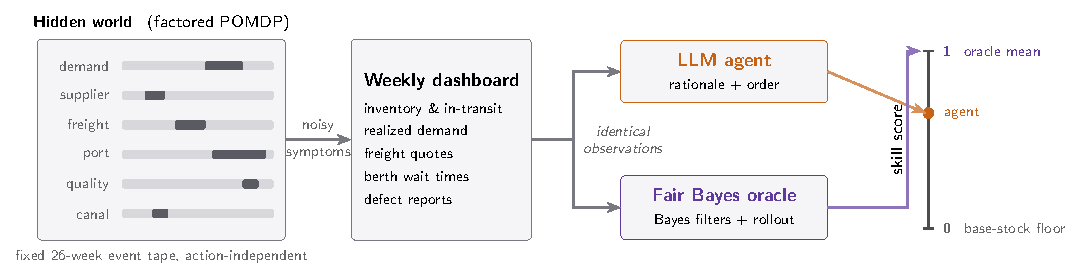
\includegraphics[width=0.85\textwidth]{figures/fig1.pdf}
  \caption{\textbf{Measuring the knowing-doing gap with a fair oracle.} Six
  hidden factor processes evolve on a fixed, action-independent event tape
  (left; dark segments mark stress regimes) and emit noisy symptoms into a
  weekly dashboard. The identical observation stream feeds both the LLM agent
  and a Bayes-filter reference policy (one exact filter per factor driving a
  rollout), so neither sees the hidden state. The agent's episode cost is
  placed on a skill scale anchored by a symptom-blind base-stock floor (0)
  and the fair oracle's 20-replication mean (1): shortfall on this scale is
  attributable to acting on beliefs, not to forming them.}
  \label{fig:overview}
\end{figure}

\section{Related Work}
\label{sec:related}

Evaluating LLM agents as sequential decision-makers has grown from
single-turn tool use into month-scale simulations of running a business.
Vending-Bench \citep{vendingbench2025} has agents operate a vending machine
across two thousand messages and finds coherence collapse, ruling out
context exhaustion as the cause. RetailBench \citep{retailbench2026}
simulates a supermarket built on real retail records, frames it as a
partially observable decision process, and finds that only a few models
survive its 180-day horizon. In inventory management specifically,
AIM-Bench \citep{aimbench2025} finds human-like ordering biases
(demand anchoring, bullwhip amplification) across five
environments, and InvAgent \citep{invagent2024} reports outcome gaps
against heuristic and reinforcement-learning baselines in a fully observed
twelve-period setting.

A second line of work asks whether agents act on what they know. In bandit
tasks, models produce a correct rationale for 87\% of decisions and still
take the greedy action over the optimal action they just derived
\citep{schmied2025greedy}. Probing studies in strategic games find internal
beliefs about the opponent that are often accurate, weakly verbalized, and
weakly linked to the chosen action \citep{sobotka2026broken}. Probes of
tool-use decisions find the same split inside the network: the belief that
an action is needed and the action taken are both linearly decodable, but
their directions drift apart in later layers \citep{cheng2026toolgap}. The
phenomenon has a name, the knowing-doing gap, and it has so far been
measured on decisions whose correct answer is known in closed form.

A third line evaluates the beliefs themselves. BayesBench
\citep{bayesbench2026} scores posterior updating against a rational Bayesian
reasoner and finds systematic departures, on estimation tasks with no
actions attached. The machinery for connecting such beliefs to inventory
decisions is classical: Bayraktar and Ludkovski
\citep{bayraktar2010inventory} derive the exact Bayes-filter reduction of
inventory control with
hidden Markov-modulated demand to a fully observed problem, in their case
to compute optimal policies.

The task is causal only in a limited sense. Causal-reasoning benchmarks test
whether a model can recover causal structure or answer interventional and
counterfactual queries \citep{cladder2023}, and there is evidence that
models recite causal facts from text rather than infer them
\citep{zecevic2023parrots}. Our task tests neither: the causal structure
of the world is given to the agent in the prompt, and actions never touch
the hidden dynamics, so there is nothing to discover and nothing to
intervene on. What the weekly decision demands is abduction, inferring
which hidden cause best explains the week's noisy symptoms under a known
model, followed by cost-sensitive control. The benchmark is
complementary to causal-reasoning evaluations: it measures whether a
correct causal attribution, once formed, survives the trip to an action.

Table~\ref{tab:related} (Appendix~\ref{app:related}) summarizes the
benchmarks closest to ours. In each,
the reference policy either reads information the agent is denied
(RetailBench's rule-based oracle takes ``structured simulator fields'' as
input; AIM-Bench's ex-post optimum is computed from realized demand) or is
absent beyond a single human run, and none grades the agent's stated
beliefs alongside its actions. STOCKTAKE addresses both limitations with
one construction: the classical filter reduction, repurposed as a reference
policy conditioned on exactly the agent's observation stream, so that
shortfall against it isolates the action side of the knowing-doing gap,
while the weekly stated beliefs it is compared against are graded on the
same episodes.

\section{STOCKTAKE: Task and Environment}

STOCKTAKE casts the agent as the replenishment manager of an electronics
importer for a 26-week episode. The state that drives cost is never
observed directly. The agent reads weekly symptoms, commits an
order, and writes down what it believes is happening
(Figure~\ref{fig:overview}).

\subsection{The weekly decision}

Each week the agent reads a dashboard of on-hand inventory, orders in
transit, realized demand, freight quotes, berth waiting times, canal
transit counts, supplier scorecards, and quality reports. It may then take
any of five within-week actions, none of which advances time.
\texttt{lock\_freight} fixes the current freight multiplier for a chosen
number of weeks; the lock itself is free, but a locked rate forgoes any
drop in the spot index. \texttt{expedite\_air} flies up to 20 units in at
\$15 per unit; they land the following week and bypass the port entirely.
\texttt{inspect\_batch} (\$40) sorts an arriving batch so that most
defective units are recovered before they stock. \texttt{buy\_briefing}
(\$30) and \texttt{buy\_audit} (\$25) reveal the true state of the canal
and of the spot supplier, respectively.

The week is then committed by exactly one call to
\texttt{place\_order(rationale, qty, route, supplier, contract)}. The
order names a quantity, a route (through the Suez Canal, or slower and
dearer around the Cape), and a supplier; the optional contract action
signs, switches, renews, or lapses a supplier contract on short, long,
strict, or lenient terms, and the agent can only source suppliers it holds
a live contract with. The \texttt{rationale} argument is required, and the
world does not advance without it. Every run therefore contains 26 written
statements of what the agent believed each week; Section~4 derives the
belief-side metrics from them.

Costs accrue for units held and in transit, for demand missed, and for the
priced levers above; the episode score is total cost, lower is better. The
price ladder is the task's core tension: sea freight is \$4 per unit and
takes three weeks, air is \$15, and every unit of missed demand costs
\$20. An agent that reads the symptoms early can buy its way out of
trouble cheaply; one that reads them late cannot.

\subsection{The hidden world}

The environment is a factored POMDP. Two structural properties of its
hidden state make a fair reference policy computable. Let $x_t = (x_t^1,
\dots, x_t^6)$ denote the hidden state in week $t$, one factor process
each for demand regime, supplier health, freight market, port congestion,
batch quality, and canal status, each a small Markov chain over
regime--age pairs that moves between a baseline and one or more stress
regimes (diagrammed in Figure~\ref{fig:world},
Appendix~\ref{app:world}). The regime and its age set the
transition probabilities: how likely a stress episode is to start, to
persist once started, and to resolve.

First, \textbf{the dynamics are factored and action-independent}. Each
factor steps as $x_{t+1}^i \sim P^i(\cdot \mid x_t^i)$, reading neither
the other factors nor the agent's action; the entire generative process
is one random stream, seeded once, consumed by the six factors in a
fixed order (Algorithm~\ref{alg:tape}, Appendix~\ref{app:world}). The
seed therefore fixes every regime change and every noisy reading for all
26 weeks before the agent exists; we call this fixed record the
episode's \emph{event tape}. Two policies run on the same seed face
byte-identical shocks and symptom noise, so the reference policies of
Section~4 are evaluated on the very tape the agent lived through.
Actions decide how much each shock costs, never what happens in the
hidden world.

The port factor instantiates the template. From clear, the port can
start building toward a backlog or take a sudden customs hold; building
tips into congested or clears; congested persists week to week until its
age cap forces recovery. Each week the realized berth wait is drawn
around the current band's mean, roughly one day when clear and sixteen
when congested, and while congested every arriving shipment is held an
extra week. The emission bands are where the benchmark's ambiguities are
constructed: for several factors the first week of two different regimes
maps to the same band, so a fresh customs hold and newly tipped
congestion both read ``slow'', and a demand promotion and a seasonal
lift both open on the same ``surge''. A single reading cannot say which
stress has begun; only the following weeks separate them.

Second, \textbf{the observations are factored}. The weekly dashboard
$o_t$ contains the fully observed logistics state (on-hand stock, orders
in transit, realized demand) and one symptom channel per factor,
$y_t^i \sim Q^i(\cdot \mid x_t^i)$. The agent never observes any $x_t^i$
directly; the paid briefing and audit of Section~3.1 are the only
exceptions, each revealing one factor's current state for a fee. The
channels themselves are hard to read in three different ways. Most are
noisy: a building port and a clear one differ by a few days of berth
wait, against scatter of the same size. The supplier scorecard is
biased, reading one severity band better than the truth by design. The
canal channel is exact but ambiguous, emitting the
same transit-count crash for a false alarm as for the first week of a real
closure, so even a Bayesian observer \emph{should} be uncertain there.

The cost function, by contrast, is \emph{not} factored. The factors
evolve independently but bill jointly through a single set of books: a
port hold delays the same shipments a demand surge is waiting on, and a
quality escape shrinks the same inventory that surge is draining.
Concurrent shocks can therefore cost far more than the same shocks
arriving in sequence, and Section~3.3 samples that regime deliberately.
Full cost constants, caps, lead times, and per-factor transition
parameters are in Appendix~\ref{app:world}.

\subsection{Seeds and stress profiles}

Because the tape is a pure function of the seed
(Algorithm~\ref{alg:tape}), instances can be minted and classified
before any agent exists. Any unsigned integer names a candidate: the
world is replayed to week 26 with empty actions, and the resulting tape
is summarized by a handful of features --- the number of stressed weeks
per factor, how many weeks have two or more factors stressed at once and
the most stressed simultaneously, the longest unbroken run of port
blockage, and whether the spot supplier failed outright. Thresholds on
these features classify the candidate's stress profile, and candidates
too benign to separate good decision-making from bad (those on which the
two reference policies of Section~4 cost nearly the same) are discarded.
The benchmark fixes fifty seeds chosen this way from a 200-seed pool:
\begin{itemize}
  \item \textsc{isolated} (12 seeds), short single-factor shocks: no
        week on the tape has two factors stressed at once;
  \item \textsc{persistent} (15 seeds), a port blockage of at least four
        consecutive weeks alongside at least four weeks of demand
        stress. Here the intuitively appealing response, freezing orders
        until the congestion clears, is the costly one, because orders
        placed \emph{through} the congestion arrive as it clears;
  \item \textsc{compound} (23 seeds), everything else: two or more
        concurrent factor episodes with no single blockage dominating
        the tape.
\end{itemize}
Compound stress is deliberately oversampled relative to the pool; it is the
regime the benchmark targets, and all results are reported per group.
The fifty seeds were curated iteratively across three rounds, screening
for stress coverage and headroom, and the persistent-profile blockage
threshold was relaxed from seven weeks to four between rounds; a
committed classifier reproduces all fifty labels from the tape features
alone, so new instances of any profile can be minted and classified with
no agent runs and no human labeling.

\subsection{Agent prompt}

Agents run under a single \emph{rules-only} prompt that specifies the
mechanics of the task (costs, lead times, levers, output format) and gives
a qualitative description of the world's factors, with no strategy advice,
no playbook, and no worked examples. The benchmark thereby measures what a
capable agent brings to the task on its own. The full
prompt and the weekly observation format are reproduced in
Appendix~\ref{app:prompt}.

\section{Experimental Setup}

\textbf{Reference policies.} Every run is scored between two reference
policies evaluated on the same seed, and both are functions of the agent's
own observation stream $o_{1:t}$, nothing more. The floor is a textbook
base-stock policy: order up to a fixed target $S = \mu L +
z\sigma\sqrt{L}$ (mean demand $\mu$, lead time $L$, safety factor $z$ from
the holding/stockout cost ratio) every week, always by the same route and
supplier, reading no symptom channel $y_t^i$ at all. The upper reference
is the Bayes-filter oracle of Figure~\ref{fig:overview}. Because the
dynamics and the observations both factor and neither reads the action
(Section~3.2), the posterior over the hidden state splits into six
independent parts, each small enough to maintain \emph{exactly}: one
forward (predict--correct) filter per factor tracks
$b_t^i = \Pr(x_t^i \mid y_{1:t}^i)$, updated each week on the same
observation dictionary $o_t$ that is serialized into the LLM prompt. To act, the oracle samples $\sim$200 possible futures of
all six factors from the belief $b_t = (b_t^1, \dots, b_t^6)$, scores a
small menu of candidate actions (order sizes, routes, each mitigation
lever, gated on the relevant posterior risk) against every sampled future,
and executes the cheapest candidate through the same action API the LLM
uses. Its randomness is independent of the world's, and it never reads
hidden state. One asymmetry is disclosed: its filters use the
environment's true generative parameters (the transition tables $P^i$ and
the regime means behind $Q^i$), which the LLM receives only as a
qualitative description. We
therefore interpret the oracle as Bayes-optimal given the true model.
Because it is a stochastic policy, its per-seed reference value is the mean
of 20 replications (standard error 0.2--1.8\% of the reference cost); it is
a fair reference rather than an optimum, and agents exceed it on some tapes
(Section~5).
Appendix~\ref{app:oracle} specifies both policies in full.

\textbf{Metrics.} Let $C_{\mathrm{base}}$, $C_{\mathrm{orc}}$, and
$C_{\mathrm{agent}}$ denote total episode cost for the floor, the oracle
reference, and the agent. The skill score
\begin{equation}
\mathrm{skill} \;=\; \frac{C_{\mathrm{base}} - C_{\mathrm{agent}}}{C_{\mathrm{base}} - C_{\mathrm{orc}}}
\end{equation}
is 0 at the symptom-blind floor and 1 at the oracle mean; values above 1 and
below 0 both occur. One of the fifty seeds has negative headroom
($C_{\mathrm{base}} < C_{\mathrm{orc}}$): the floor already beats the oracle
mean on that tape, so skill is undefined there, and the seed is excluded
from every skill mean (leaving $n = 49$). Its runs still count in a
denominator-free companion statistic, the number of seeds on which the
agent's raw cost beats the floor's. Three further seeds have headroom under
\$700, where the ratio is noisy; they are flagged in the per-seed results
but not excluded. A worked example from seed~1: base-stock costs \$9{,}101,
the oracle mean is \$6{,}932, and Claude Sonnet 5 spent \$8{,}539, so its
skill is $(9101-8539)/(9101-6932)=0.26$. For belief-side metrics, a
\emph{stress episode} is a maximal run of consecutive weeks in which one
factor is truly in a stress regime (283 episodes per model across the
fifty tapes, of which 266 are detectable: seventeen begin in the final
week, after the last rationale is written, and are excluded from the
detection denominator rather than counted as missed; the final week's
stress weeks are likewise excluded from the diagnosed/undiagnosed pools,
since no rationale exists to judge them by).
Detection lag is the number of weeks from episode onset until the factor is
first named in the agent's rationale (averaged over detected episodes;
never-detected episodes are reported separately), and the knowing-doing rate
is
\begin{equation}
\mathrm{KD} \;=\; \Pr\!\left(\,\text{stockout in week } t \;\middle|\; \text{a truly stressed factor is named in week } t\,\right),
\end{equation}
estimated over the group's correctly diagnosed stress weeks, where
``stockout'' means the world served less than that week's realized demand
--- an actual shortfall on the engine's books.\footnote{An earlier version
of this metric re-derived the stockout flag from the trace's printed
inventory arithmetic, which omits air-expedited arrivals; 343 weeks that
air freight saved were miscounted as stockouts, inflating every
knowing-doing rate, most for the heaviest air users. All belief-side
stockout figures here are recomputed from the engine replay of
Table~\ref{tab:decomp}. Detection and lag never read this flag and are
unaffected.} A high KD rate means correct diagnosis coexisting with empty
shelves.

\textbf{Belief grading.} Whether a rationale names a factor is judged by a
small LLM grader (gpt-5-mini, temperature 0) that sees only the rationale
text and the fixed factor vocabulary, never the tape; labels are aligned to
the week the rationale was written. Grader labels were audited in two rounds
against raw traces; residual disagreements are borderline over-labels on calm
weeks, which cannot enter the knowing-doing rate by construction. The rationale is stated
belief: a lower bound on what the model knows, a point we return to in
Section~6. Grading rules and validation details are in
Appendix~\ref{app:grading}.

\textbf{Models.} We evaluate Claude Sonnet 5, GPT-5.4, DeepSeek-V4-Pro,
and Grok 4.5, each on all fifty seeds. All four run through an identical
harness (OpenRouter model IDs \texttt{anthropic/claude-sonnet-5},
\texttt{openai/gpt-5.4}, \texttt{deepseek/deepseek-v4-pro},
\texttt{x-ai/grok-4.5}; temperature 0; runs completed July 2026), one run
per model--seed pair, 200 episodes in total, each validated to the full 26
weeks, all under the rules-only prompt of
Section~3.\footnote{An earlier circulated draft reported DeepSeek-V4-Pro
on a twenty-seed subset after a belief-grading fault silently read stale
run files; all numbers here are from complete fifty-seed runs, regraded
and rescored.}

\section{Results}

\begin{figure}[t]
  \centering
  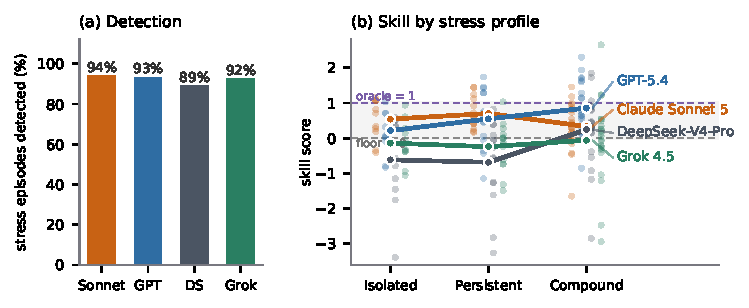
\includegraphics[width=0.85\textwidth]{figures/fig2.pdf}
  \caption{\textbf{Seeing is uniform; doing is not.} (a) All four models
  detect 89--94\% of their detectable hidden-factor stress episodes (266
  per model over the fifty seeds; seventeen more begin in the final week,
  after the last rationale, and are excluded rather than counted as
  missed), typically within a week of onset. (b) Group-mean
  skill by stress profile (lines), with per-seed scores as faint dots.
  Costs diverge across models despite panel (a): DeepSeek-V4-Pro and
  Grok 4.5 finish below the symptom-blind floor overall.}
  \label{fig:results}
\end{figure}

\begin{table}[t]
  \caption{Skill score by stress profile: group mean (median), single run
  per model--seed pair, every model on all fifty seeds (11/15/23 scoreable
  per group after the seed with negative headroom is excluded). \emph{neg}
  counts scoreable seeds below the base-stock floor; \emph{beats floor}
  counts every seed, including the excluded one, on which the agent's raw
  cost beat the floor's.}
  \label{tab:skill}
  \centering
  \small
  \begin{tabular}{lcccccc}
    \toprule
    Model & \textsc{isolated} & \textsc{persistent} & \textsc{compound} & All & neg & beats floor \\
    \midrule
    Claude Sonnet 5 & 0.54 (0.71) & 0.70 (0.61) & 0.33 (0.35) & 0.49 (0.45) & 9 & 40/50 \\
    GPT-5.4         & 0.21 (0.07) & 0.55 (0.61) & 0.86 (0.73) & 0.62 (0.65) & 8 & 42/50 \\
    DeepSeek-V4-Pro & $-$0.62 ($-$0.57) & $-$0.68 ($-$0.26) & 0.24 (0.32) & $-$0.23 (0.15) & 22 & 28/50 \\
    Grok 4.5        & $-$0.14 ($-$0.32) & $-$0.24 ($-$0.12) & $-$0.06 (0.05) & $-$0.13 ($-$0.08) & 28 & 21/50 \\
    \bottomrule
  \end{tabular}
\end{table}

\begin{table}[t]
  \caption{Belief-side metrics. Detection is pooled over each model's
  stress episodes; the knowing-doing rate is the fraction of correctly
  diagnosed stress weeks that still ended in stockout, pooled over the
  group's stress weeks (week counts in parentheses; the final week's
  stress weeks are excluded as unknowable --- no rationale exists to
  judge them by). The last column is the severity-confound check: the
  stockout rate on stress weeks the model failed to diagnose. Diagnosed
  weeks stock out more than undiagnosed ones for every model
  (Holm-adjusted $p \le 0.022$), so part of the knowing-doing rate
  reflects severity rather than inaction.}
  \label{tab:belief}\label{tab:confound}
  \centering
  \small
  \begin{tabular}{lccccccc}
    \toprule
    & \multicolumn{2}{c}{Detection} & \multicolumn{4}{c}{Knowing-doing rate} & Confound \\
    \cmidrule(lr){2-3}\cmidrule(lr){4-7}\cmidrule(lr){8-8}
    Model & missed & mean lag (wk) & \textsc{isol.} & \textsc{persist.} & \textsc{comp.} & all & undiag. \\
    \midrule
    Claude Sonnet 5 & 16/266 & 0.42 & 0.10 & 0.22 & 0.18 & 0.18 (515) & 0.06 (124) \\
    GPT-5.4         & 18/266 & 0.40 & 0.05 & 0.18 & 0.08 & 0.11 (502) & 0.04 (137) \\
    DeepSeek-V4-Pro & 29/266 & 0.32 & 0.05 & 0.26 & 0.14 & 0.17 (469) & 0.02 (170) \\
    Grok 4.5        & 20/266 & 0.32 & 0.06 & 0.18 & 0.13 & 0.14 (544) & 0.02 (95) \\
    \bottomrule
  \end{tabular}
\end{table}

All four models see the hidden world about equally well
(Table~\ref{tab:belief}, Figure~\ref{fig:results}a). Each detects 89--94\% of
its detectable stress episodes, with a mean lag of 0.32--0.42 weeks: when a factor
enters a stress regime, its symptoms are typically named in the rationale
within the same week. The two models that end up below the base-stock
floor on cost detect no slower than the two that beat it. Whatever separates
these models on this task, it is not state estimation.

Skill scores, in contrast, diverge widely (Table~\ref{tab:skill},
Figure~\ref{fig:results}b). Claude Sonnet 5 and GPT-5.4 recover 49\% and
62\% of the floor-to-oracle cost gap overall and beat the base-stock
floor's raw cost on 40 and 42 of 50 seeds. DeepSeek-V4-Pro and Grok 4.5
score $-0.23$ and $-0.13$, falling below the floor on 22 and 28 of their
49 scoreable seeds: on roughly half their tapes, a symptom-blind
base-stock rule with the same action menu would have been cheaper than
acting on their (largely correct) diagnoses. Along the stress axis the
field splits three against one. GPT-5.4, DeepSeek-V4-Pro, and Grok 4.5
all post their best group on \textsc{compound} seeds (GPT-5.4 strongest
at 0.86, with its weakest group \textsc{isolated} at mean 0.21, median
0.07), while Claude Sonnet 5 is the exception: strongest on
\textsc{persistent} (0.70, no seed below the floor) and weakest on
\textsc{compound}, where seven of its nine below-floor seeds sit.
DeepSeek's \textsc{compound} mean is pulled up by a single outlier tape;
its group median is 0.32. Individual scores above 1 occur (33 of 196
scoreable runs) and are legitimate, since the oracle is Bayes-optimal in
expectation but not per-tape. Even the best model leaves over a third of
the floor-to-oracle gap unrecovered, so the benchmark is far from
saturated.

\paragraph{Uncertainty.} Because every model runs the same fifty seeds, we
quantify uncertainty with a paired design over the 49 scoreable seeds:
$10^4$-draw paired bootstrap for 95\% confidence intervals and Wilcoxon
signed-rank tests on per-seed differences, Holm-corrected within each
family of comparisons. Mean skill is $0.62\ [0.40, 0.83]$ for GPT-5.4,
$0.49\ [0.32, 0.65]$ for Claude Sonnet 5, $-0.13\ [-0.39, 0.12]$ for
Grok 4.5, and $-0.23\ [-0.57, 0.08]$ for DeepSeek-V4-Pro. The picture that
survives testing is a \emph{two-tier} one: every cross-tier contrast is
significant (Holm-adjusted $p \le 2\times10^{-4}$), while neither
within-tier ordering is (GPT-5.4 vs.\ Claude Sonnet 5, $p = 0.26$;
Grok 4.5 vs.\ DeepSeek-V4-Pro, $p = 0.80$). The two bottom-tier means are
statistically indistinguishable from the symptom-blind floor itself
($p = 0.33$ and $0.56$): the supported claim is that they fail to beat a
rule that ignores every symptom, not that they reliably fall below it. Of
the \textsc{compound} exception, only the GPT-5.4 side is significant
(Claude Sonnet 5 trails it by 0.53 there, Holm $p = 0.001$); Sonnet's
deficit against the two bottom-tier models on \textsc{compound} is not.
The median half-width of a pairwise-contrast interval, 0.31 skill units,
is the benchmark's effective resolution at fifty seeds: single runs
separate tiers, not neighbors. Noise from the oracle reference itself is
negligible --- propagating its per-seed standard error moves a skill score
by a median of 0.02, against a seed-to-seed spread of 0.6--1.2. The same
machinery applied to the belief side (seed-cluster bootstrap over each
model's fifty seeds) grades those claims too. No pairwise difference in
detection rate survives correction (smallest Holm-adjusted $p = 0.05$), so
we describe detection as uniform in the sense of no detectable difference,
not proven equality. The apparent lag ordering --- the two bottom-tier
models naming factors fastest --- dissolves entirely (all Holm-adjusted
$p = 1.0$); the supported statement is that they detect \emph{no slower}.
On the corrected stockout flags (see the footnote in Section~4), the
knowing-doing peak on \textsc{persistent} seeds holds in point estimate
for all four models but is significant for two (GPT-5.4 and
DeepSeek-V4-Pro, Holm-adjusted $p = 0.018$ and $0.028$), and the severity
confound of Table~\ref{tab:confound} is significant for all four models
(Holm-adjusted $p \le 0.022$) once the final week's unknowable stress
weeks leave the undiagnosed pool.

The knowing-doing rate (Table~\ref{tab:belief}) shows where correct diagnosis
fails to prevent empty shelves. The rate peaks on
\textsc{persistent} seeds in point estimate for every model, at 0.18--0.26
versus 0.05--0.10 on \textsc{isolated} seeds, though the peak reaches
significance for two of the four (GPT-5.4 and DeepSeek-V4-Pro, Holm
$p = 0.018$ and $0.028$; Claude Sonnet 5 and Grok 4.5, $p = 0.23$): when a
disruption lasts many weeks, roughly one correctly diagnosed stress week
in five still ends in stockout.
Brief shocks are handled; sustained ones convert knowledge into cost, and
a pre-registered check attributes the peak to duration rather than to the
profile label: per-seed rates rise with the longest port blockage
(Spearman $+0.36$ to $+0.62$, Holm $p \le 0.015$, for three of the four
models, GPT-5.4 positive but not significant), while \textsc{persistent}
membership adds no detectable association once blockage duration is
controlled (Holm $p \ge 0.086$ for all four).
The rate is not a model ranking, however, and it does not track skill in
either direction: the highest rate belongs to the second-best model
(Claude Sonnet 5, 0.18) and the lowest to the best (GPT-5.4, 0.11). The
reason is that a
stockout-based rate sees only one face of the gap. An agent can fail on a
correct diagnosis by under-responding, stocking out despite naming the
problem, or by over-responding, buying so much protection that
stockouts are rare while the bill exceeds what the symptom-blind floor
would have paid. The two models below the floor show stockout rates
between the leaders', while their diagnosed-week totals are the highest
of the four. A per-week cost decomposition of all
four models (below) measures which face each model shows and through
which instrument. Two further qualifications keep
the rate from reading as a week-level fault measure. A
stockout in a given week can stem from an ordering decision made weeks
earlier. And Table~\ref{tab:confound} shows a severity confound: weeks
bad enough to be noticed are also bad enough to strain the shelf,
for every model. The knowing-doing rate therefore
says that correct diagnosis does not guarantee protection; it does not say
that diagnosis causes stockouts, and we do not rank models on it.

Reading the traces suggests the models fail in opposite directions; full
excerpts are in Appendix~\ref{app:seeds}, and Figure~\ref{fig:seed1}
plots the first episode. Claude Sonnet 5 on seed~1 (\textsc{persistent};
port congested weeks 17--24 while demand lifts) \emph{freezes}: it
diagnoses the congestion in week~16 and skips its sea order at once, and
through weeks 22--24, at zero inventory, it stops ordering by sea
entirely, counting the 104 units trapped behind the congestion it itself
diagnosed as reason enough (``an already oversized pipeline''). It ends
with four consecutive zero-inventory weeks costing \$660--\$823 each, while
the oracle keeps placing modest orders that arrive after the congestion
clears. DeepSeek-V4-Pro on seed~25 (\textsc{isolated}; a two-week canal
closure) \emph{flails}: within two weeks of a correct diagnosis it locks
freight rates for four weeks, air-expedites units, and stacks 80 units of
orders against $\sim$20-per-week demand, on top of 117 already in
transit. The closure ends in week~5; the fees and holding costs it bought
persist, and the episode finishes at skill $-1.45$. Neither trace contains
a detection error. The two directions generalize beyond these seeds. In
every one of Claude Sonnet 5's nine below-floor seeds, its spending on
air expedite alone exceeds its entire excess over the floor, and about
nine in ten of its air orders on those seeds coincide with a genuine
disruption: it over-doses real problems rather than chasing noise.
GPT-5.4 errs the other way, structurally under-using the mitigation
levers: it never locks freight rates in 87\% of the seeds containing a
freight spike and never orders a batch inspection in 63\% of the seeds
with quality escapes, while naming those conditions in its rationales.

\begin{table}[t]
  \centering
  \small
  \begin{tabular}{lrrrrrr}
    \toprule
    Model & $n$ wk & Procure & Holding & Stockout & Levers & Incident \\
    \midrule
    GPT-5.4 & 502 & 61 [49,75] & 98 [93,104] & 20 [11,31] & 91 [76,107] & 30 [21,40] \\
    \quad\emph{oracle, same weeks} & & \emph{65 [57,75]} & \emph{95 [92,98]} & \emph{37 [25,50]} & \emph{58 [43,75]} & \emph{34 [24,44]} \\
    Claude Sonnet 5 & 515 & 70 [61,79] & 85 [81,88] & 32 [23,42] & 126 [110,142] & 29 [21,38] \\
    \quad\emph{oracle, same weeks} & & \emph{65 [57,73]} & \emph{95 [92,98]} & \emph{34 [23,45]} & \emph{55 [40,70]} & \emph{32 [23,41]} \\
    Grok 4.5 & 544 & 87 [77,96] & 120 [113,128] & 37 [24,52] & 81 [66,96] & 40 [29,53] \\
    \quad\emph{oracle, same weeks} & & \emph{67 [58,76]} & \emph{95 [92,98]} & \emph{33 [23,44]} & \emph{57 [41,73]} & \emph{32 [23,42]} \\
    DeepSeek-V4-Pro & 469 & 98 [83,114] & 133 [121,145] & 37 [27,48] & 67 [51,83] & 45 [32,60] \\
    \quad\emph{oracle, same weeks} & & \emph{68 [59,78]} & \emph{95 [92,98]} & \emph{37 [26,49]} & \emph{60 [43,77]} & \emph{35 [25,46]} \\
    \bottomrule
  \end{tabular}
  \caption{Cost decomposition of correctly diagnosed stress weeks: mean
  \$/week per component from replaying every logged action through the
  world engine (the replay reproduces all 5{,}200 logged weekly totals
  exactly). Italic rows: the fair oracle's spend on the same (seed, week)
  cells under its 20-replication protocol. Brackets: 95\% seed-cluster
  bootstrap intervals. Procure = shipping plus diversion surcharge;
  holding includes capital cost on in-transit units; stockout includes
  backorder coupling; levers = air, inspection, briefing, audit,
  dual-sourcing; incident = demurrage plus rework.}
  \label{tab:decomp}
\end{table}

The decomposition in Table~\ref{tab:decomp} turns those trace readings into
measurement. Every model escalates once it diagnoses stress: premium-lever
spending on diagnosed weeks exceeds the same model's calm-week level by
\$42--\$87 per week (Holm-adjusted $p < 10^{-4}$ for each of the four), so
the gap is a matter of instrument and dose, never of sitting still. Claude
Sonnet 5 buys the most protection, \$126 per diagnosed week with \$116 of
it air freight, and its air spending exceeds GPT-5.4's by \$31 [13, 50] per
week (Holm $p < 10^{-4}$) --- the measured form of the over-dosing in
Exhibit~A. GPT-5.4's lever spending is almost entirely air as well (\$86 of
\$91); the targeted levers it skips, rate locks and inspections, are cheap
enough that its under-use shows up in counts, not dollars. For the two
bottom-tier models the lever bucket, \$81 and \$67 per diagnosed week, is
not where their cost concentrates: ordering and carrying dominate
(procurement \$87 and \$98, holding \$120 and \$133 per week), and their
holding runs \$115--\$129 per week even on calm weeks. Measured,
their over-response is bulk over-ordering and stock carried against
$\sim$20-per-week demand, with premium fees a secondary channel.
The oracle rows turn that composition into excess. The fair oracle spends
\$55--60 per week on levers during those same diagnosed weeks, so
escalating is what a competent policy does there; the models' defect is
dose and instrument. Against that reference, the pre-registered contrasts
land as predicted for the two below-floor models: Grok 4.5 and
DeepSeek-V4-Pro hold \$25 [18, 34] and \$38 [26, 50] more per diagnosed
week than the oracle, and spend \$20 [8, 31] and \$30 [14, 47] more on
procurement (Holm $p \le 0.0012$ for all four contrasts). Claude Sonnet
5's air spending runs \$65 [49, 83] per week above the oracle's on its
diagnosed weeks (Holm $p < 10^{-4}$), while its holding came out
\emph{below} the oracle's ($-\$10$ [$-14$, $-6$]), the opposite sign
from our pre-registration, and GPT-5.4 differs from the oracle on
neither bucket at our resolution. Because week-$t$ books carry each
policy's earlier decisions, these are comparisons on the same tape
weeks, not per-decision counterfactuals. One
pre-registered expectation failed in the opposite direction: we expected
GPT-5.4's diagnosed-week cost to be more stockout-shaped than Sonnet's,
and its stockout share is in fact the lower of the two (difference
$-0.03$ [$-0.06$, $-0.004$], $p = 0.026$).

\section{Discussion and Limitations}
\label{sec:discussion}

The results support one claim: on this task, frontier-model failures are
concentrated in control, not state estimation, and the fair oracle makes that
split measurable. A privileged oracle could not have licensed it, because any
shortfall could be attributed to the information gap rather than to policy.
The fairness carries the one asymmetry disclosed in Section~4 --- the
oracle's filters use the true generative parameters, the LLM only a
qualitative world description --- so skill~$=1$ means ``Bayes-optimal
given the true model'', and scores above 1 are possible and observed.

The knows-the-physics half of that asymmetry is testable, and we test it.
We refit every transition probability of the six factor chains by
Baum--Welch expectation--maximization \citep{rabiner1989hmm} on 200
passively observed episodes (seeds disjoint from the benchmark's;
observation streams only, with the sensor model, state topology, and cost
mechanics held known), then reran the full reference protocol with the
learned tables in place of the true ones. The learned reference differs
from the true one by $+\$71\ [-\$20, +\$186]$ per seed (1.2\% of the mean
reference cost; Wilcoxon $p = 0.47$): a reference that learned its
dynamics from watching is statistically indistinguishable from the one
that was given them, with plausible degradation capped at three percent.
Re-scoring all four models against the learned reference shifts mean
skill by $+0.04$ to $+0.10$, every interval straddling zero and inside
the benchmark's 0.31 resolution, so the two-tier structure is unchanged;
one seed flips to negative headroom and drops out. The fit is imperfect
where the data are thin: the quality chain's deep drifting-age hazards
stay badly estimated (deep ages are rarely visited and the
accept/marginal/reject inspection channel carries no age signal), and the
largest cost gaps land exactly where that predicts, on quality-stressed
and \textsc{compound} seeds, without reaching significance there either.
What stays privileged is stated: emission parameters and the planner's
cost model are still read from the configuration, and the passive tapes
lack the realized-fill channel a deployed oracle sees when it orders.

The belief metrics read stated beliefs, and stated belief is a lower bound.
Detection is measured from the rationale the model writes, not from its
internal state; a model may track a factor it never mentions. This biases
detection down, which strengthens the seeing-vs-doing contrast, but the
knowing-doing rate inherits the grader's labels. A stratified manual read
found the labels correct on the sampled metric-relevant weeks; an
independent second grader agrees with the production grader on the
metric-relevant component (which named factors intersect true stress) at
89\%, with residual disagreement on calm-week over-labels, which cannot
enter the knowing-doing rate by construction. Both audits sampled the
original twenty-seed grading run; later grading used the identical
configuration but was not freshly audited. Three further reading rules
come from adversarial checks of the grading pipeline (each check, its
fix, and the numbers it moved are logged in the released defect ledger).
Detection rewards recall only: naming precision is 0.29--0.35 for all
four models against at-threshold stress, rising to 0.36--0.43 when
namings of real but sub-threshold activity (a tightening freight market,
a wobbling supplier) are not counted against it. On weeks with several
simultaneous stresses, the any-overlap rule counts a partial diagnosis as
diagnosed (55--70\% of such diagnosed weeks named only a subset); under a
stricter full-coverage rule the \textsc{persistent} peak persists exactly
for the two models where it is significant. And the remaining misses are
mostly right-censored: of the 16--29 never-detected episodes per model,
9--17 begin in weeks 24--25 with one or two rationales left to catch them
--- a hard tail that every model faces equally.

Two design choices qualify behavioral readings of the traces. A signed
second supplier contract cannot be ended (the lapse action affects only
unsigned offers), so the weekly dual-sourcing fee is unavoidable from
that point for every agent, and paying it is not by itself a decision
error. And the paid audit and briefing return near-deterministic ground
truth by design, so what varies across models is how often they are
consulted, not how well their output is read.

The cost-side numbers rest on single runs: each model--seed cell is one
run, and provider-side nondeterminism is unquantified. Group means pool
11--23 seeds, and the cross-model contrasts (a 0.85-point overall skill
spread against detection rates within four points of one another) are far
larger than plausible single-run noise, but per-seed values should be
read as samples, not estimates.

Finally, the benchmark covers one domain, one SKU, one prompt arm, and
four models. The tapes are generated from published seeds rather than
scraped, so they cannot occur in training data, but conclusions about
\emph{why} the gap concentrates on persistent stress await intervention:
prompt arms that coach explicit belief maintenance, repeated runs per cell,
a clairvoyant ceiling to bound the oracle's optimality gap, and a broader
model set.

\begin{thebibliography}{99}
\small

\bibitem{vendingbench2025}
A.~Backlund and L.~Petersson.
Vending-Bench: A benchmark for long-term coherence of autonomous agents.
arXiv:2502.15840, 2025.

\bibitem{retailbench2026}
L.~Zhang, J.~Wang, J.~Wu, and Z.~Zhang.
RetailBench: Evaluating long-horizon autonomous decision-making and strategy
stability of LLM agents in realistic retail environments.
arXiv:2603.16453, 2026.

\bibitem{aimbench2025}
X.~Zhao, Y.~Xie, C.~Chen, and Y.~Sun.
AIM-Bench: Evaluating decision-making biases of agentic LLM as inventory
manager.
arXiv:2508.11416, 2025.

\bibitem{invagent2024}
Y.~Quan and Z.~Liu.
InvAgent: A large language model based multi-agent system for inventory
management in supply chains.
arXiv:2407.11384, 2024.

\bibitem{schmied2025greedy}
T.~Schmied, J.~Bornschein, J.~Grau-Moya, M.~Wulfmeier, and R.~Pascanu.
LLMs are greedy agents: Effects of RL fine-tuning on decision-making
abilities.
arXiv:2504.16078, 2025.

\bibitem{sobotka2026broken}
J.~Sobotka, M.~O.~Karabag, and U.~Topcu.
Why do LLMs struggle in strategic play? Broken links between observations,
beliefs, and actions.
arXiv:2605.00226, 2026.

\bibitem{cheng2026toolgap}
Y.~Cheng, C.~Fan, M.~JafariRaviz, K.~Rezaei, and S.~Feizi.
Model-adaptive tool necessity reveals the knowing-doing gap in LLM tool
use.
arXiv:2605.14038, 2026.

\bibitem{cladder2023}
Z.~Jin, Y.~Chen, F.~Leeb, L.~Gresele, O.~Kamal, Z.~Lyu, K.~Blin,
F.~Gonzalez~Adauto, M.~Kleiman-Weiner, M.~Sachan, and B.~Sch\"olkopf.
CLadder: Assessing causal reasoning in language models.
arXiv:2312.04350, 2023. NeurIPS 2023.

\bibitem{zecevic2023parrots}
M.~Ze\v{c}evi\'c, M.~Willig, D.~S.~Dhami, and K.~Kersting.
Causal parrots: Large language models may talk causality but are not
causal.
arXiv:2308.13067, 2023.

\bibitem{bayesbench2026}
A.~Samanta, A.~Magesh, T.~Lancewicki, A.~Jain, Y.~Yu, P.~Sajda, K.~Hassani,
A.~Modi, D.~R.~Jiang, and Y.~Efroni.
BayesBench: Evaluating LLM belief trajectories under multi-turn evidence
accumulation.
arXiv:2606.30850, 2026.

\bibitem{bayraktar2010inventory}
E.~Bayraktar and M.~Ludkovski.
Inventory management with partially observed nonstationary demand.
\emph{Annals of Operations Research}, 176(1):7--39, 2010.

\bibitem{rabiner1989hmm}
L.~R.~Rabiner.
A tutorial on hidden Markov models and selected applications in speech
recognition.
\emph{Proceedings of the IEEE}, 77(2):257--286, 1989.

\end{thebibliography}

\newpage
\appendix
\section*{Appendix}

\section{Benchmark Comparison}
\label{app:related}

\begin{table}[h]
  \caption{The benchmarks closest to STOCKTAKE (Section~2). Cells condense
  each paper's own description of its task and reference policies;
  citations in the main text. RetailBench builds its simulator from real
  retail records; ours is synthetic and seeded.}
  \label{tab:related}
  \centering
  \small
  \setlength{\tabcolsep}{5pt}
  \begin{tabular}{@{}l >{\raggedright\arraybackslash}p{2.0cm} >{\raggedright\arraybackslash}p{1.6cm} >{\raggedright\arraybackslash}p{2.9cm} >{\raggedright\arraybackslash}p{3.1cm} l@{}}
    \toprule
    Benchmark & Setting & Horizon & Hidden state & Reference policy & Belief graded \\
    \midrule
    Vending-Bench & vending machine & 2{,}000 messages & per-step noise only & none (human baseline) & no \\
    AIM-Bench & five inventory envs & 20 rounds (NVP); varies & stochastic demand, lead times & hindsight optimum & no \\
    RetailBench & retail store sim & 180 days & news-impact and supplier params & rule-based, privileged & no \\
    \midrule
    \textbf{STOCKTAKE} & import replenishment & 26 weeks & six persistent factor processes & Bayes-filter rollout on the agent's observations & yes \\
    \bottomrule
  \end{tabular}
\end{table}

\section{World and Cost Parameters}
\label{app:world}

All values below are read directly from the environment source; they fully
specify the weekly cost function and the six hidden factor processes of
Section~3, diagrammed in Figure~\ref{fig:world}.

\begin{figure}[h]
  \centering
  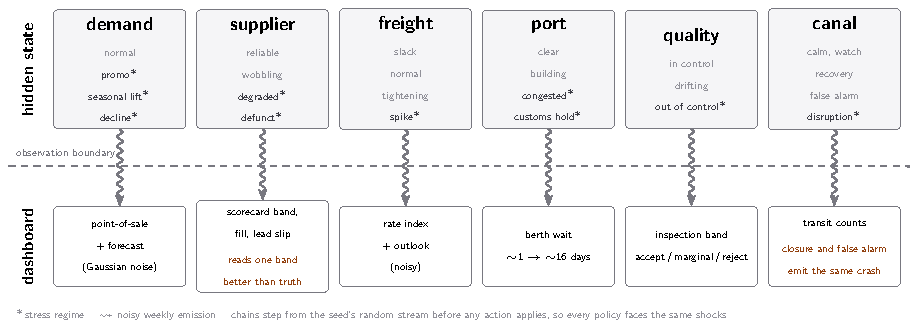
\includegraphics[width=0.88\textwidth]{figures/fig_world.pdf}
  \caption{The hidden world behind the dashboard. The hidden state is six
  independent Markov chains; starred regimes are the stress regimes that
  define episodes in Section~4. Each chain emits one symptom stream
  into the weekly dashboard, and those streams are all the agent (and the
  oracle) ever sees. Two symptoms mislead by construction (orange): the
  supplier scorecard reads one severity band better than the truth, and
  the canal's transit counts crash identically for a real closure and a
  false alarm.}
  \label{fig:world}
\end{figure}

\begin{algorithm}[h]
\caption{Event-tape generation. One random stream $r$, seeded once, is
consumed by the six factors in a fixed order; no step reads an agent
action, so the tape is a pure function of the seed. Lines 5--10 are the
transition kernel $P^i$ and line 11 the emission kernel $Q^i$ of
Section~3.2; every onset rate, persistence rate, age cap, and band mean
is tabulated below. A few factors draw auxiliary state from the same
stream in the same fixed order, such as the canal event's type at onset.}
\label{alg:tape}
\begin{algorithmic}[1]
\State $r \gets \textsc{Random}(\mathit{seed})$
\State $(s^i, a^i) \gets (\text{baseline}^i,\, 0)$ for each factor $i$ \Comment{regime and its age}
\For{week $t = 1, \dots, 26$}
  \For{factor $i$ in fixed order} \Comment{canal, supplier, demand, freight, port, quality}
    \If{$s^i$ is the baseline}
      \State leave it for regime $k$ w.p.\ $\mathrm{onset}^i_k$, else stay \Comment{e.g.\ clear $\to$ building}
    \Else
      \State stay w.p.\ $\mathrm{persist}^i(s^i, a^i)$, else advance a stage or recover \Comment{forced out at $\mathrm{cap}^i(s^i)$}
    \EndIf
    \State $a^i \gets a^i{+}1$ if the regime held, else $0$; \quad $x_t^i \gets (s^i, a^i)$
    \State $y_t^i \gets$ factor $i$'s readings, drawn from $r$ around its band's mean \Comment{e.g.\ $\mathrm{round}\,\mathcal{N}(\mu_{\text{band}}, \sigma)$}
  \EndFor
\EndFor
\State \Return the tape $(x_{1:26},\, y_{1:26})$
\end{algorithmic}
\end{algorithm}

\paragraph{Costs.} Each week's cost is the sum of the applicable components:

\begin{center}
\small
\begin{tabular}{lll}
\toprule
Component & Charge & When \\
\midrule
Sea shipping & \$4.00 (Suez) / \$6.00 (Cape) per unit $\times$ freight mult. & at dispatch \\
Supplier price delta & qualified $+$\$1.00, spot $-$\$1.50, backup $+$\$0.30 per unit & at dispatch \\
Holding & \$1.00 per unit-week, on hand and in transit & weekly \\
Stockout & \$20.00 per unit of unmet demand (lost sales) & weekly \\
Port demurrage & \$2.00 per unit held at a blocked port & while blocked \\
Quality rework & \$15.00 per defective unit landed & at arrival \\
Diversion surcharge & \$2.00 per unit forced from Suez around the Cape & at diversion \\
Crisis back-order & \$60.00 per unit a supplier shorts during a canal event & coupled \\
Air expedite & \$15.00 per unit, at most 20 units/week & on use \\
Briefing / audit / inspection & \$30 / \$25 / \$40 flat per call & on use \\
Dual-sourcing overhead & \$4.00 per week while two or more contracts are live & weekly \\
\bottomrule
\end{tabular}
\end{center}

Orders are capped at 100 units per week. Sea lead times are 3 weeks via
Suez and 4 via the Cape; air freight lands the following week. The implied
newsvendor critical ratio is $20/21 \approx 0.95$, which fixes the
base-stock safety factor $z \approx 1.67$ used by the floor policy.

\paragraph{Factor processes.} Each factor is an independent Markov chain
stepped from the seed's random stream before any action applies. Starred
regimes are the stress regimes that define episodes in Section~4.

\begin{center}
\small
\begin{tabular}{lp{4.6cm}p{6.2cm}}
\toprule
Factor & Regimes & Key dynamics and observations \\
\midrule
Demand & normal, promo spike$^{*}$, seasonal lift$^{*}$, structural decline$^{*}$ &
onsets 0.03/0.015/0.005 per week; promo lasts 4 weeks, seasonal persists 0.85
(cap 8), decline persists 0.97. Weekly means 20/26/30/14 units; observed
point-of-sale and forecast carry Gaussian noise (sd 4 and 6). \\
Supplier & reliable, wobbling, degraded$^{*}$, defunct$^{*}$ &
onset 0.10, wobbling$\to$degraded 0.45; degraded recovers within 4 weeks or
dies (0.06). Scorecard band reads one severity level better than the truth;
lead-time slip and fill fraction are noisy. \\
Freight & slack, normal, tightening, spike$^{*}$ &
tightening onset 0.06, tightening$\to$spike 0.18, spike persists 0.80 (cap
6). Rate multipliers 0.7/1.0/1.8/4.0; index and outlook noisy. \\
Port & clear, building, congested$^{*}$, customs hold$^{*}$ &
building onset 0.06, building$\to$congested 0.30, congested persists 0.85
(cap 8); customs holds last about a week. Berth wait rises from $\sim$1 to
$\sim$16 days; a blocked port delays every arrival one week. \\
Quality & in control, drifting, out of control$^{*}$ &
drift onset 0.04; the drift-to-failure hazard grows with age
($0.05 + 0.04 \cdot \text{age}$). Defect fractions 0.1\%/2\%/6\%; observed
only as a noisy accept/marginal/reject inspection band. \\
Canal & calm, watch, disruption$^{*}$, recovery, false alarm &
calm$\to$watch 0.08; watch resolves to a real closure (0.50) or a false
alarm (0.20). Transit counts are exact but the first closure week and a
false alarm emit the identical ``crash'' reading. A closed canal queues
Suez ships, then diverts them ($+$3 weeks, Cape rate, surcharge). \\
\bottomrule
\end{tabular}
\end{center}

\section{Reference Policy Details}
\label{app:oracle}

\paragraph{Base-stock floor.} Order-up-to level
$S = \mu L + z\sigma\sqrt{L}$ with $\mu = 20$, $\sigma = 4$, $L = 4$ (3-week
Suez lead plus one review week), $z = \Phi^{-1}(20/21) \approx 1.67$. Every
week it orders $\max(0, S - \text{inventory position})$, always via Suez
from the same supplier, and never touches a lever or reads a symptom.

\paragraph{Oracle decision loop.} Each week the oracle (i) updates one exact
forward Bayes filter per factor on the shared observation dictionary;
(ii) samples $\sim$200 joint futures of all six factors from the filter
posteriors, rolled forward to the episode's final week with the true
transition tables; (iii) scores a
small candidate menu against every sampled future using a fast surrogate of
the cost function, holding future weeks to a base-stock continuation; and
(iv) executes the cheapest candidate through the world's action methods,
the same calls that back the LLM's tools. The candidate menu contains order quantities \{0, four weeks, six
weeks of expected demand\}, both routes, the contracted suppliers, and each
mitigation lever gated on posterior risk (freight lock if
$\Pr(\text{tightening or spike}) > 0.3$; air expedite if port risk $> 0.3$;
inspection if quality risk $> 0.5$ and a batch lands next week). The same
sampled futures are reused across candidates (common random numbers). The
oracle never buys briefings or audits; the LLM may. A seed's reference
value is the mean of 20 such runs; replications vary both the random
stream and the per-decision trajectory budget (191--210 sampled futures,
hence the $\sim$200).

\section{Belief Grading Details}
\label{app:grading}

The grader (gpt-5-mini via OpenRouter, temperature 0, reasoning effort
capped at low) receives only the week's rationale text and the fixed
six-name factor vocabulary, and returns strict JSON. Its instructions require a
factor to be labeled only if the text claims it is a problem \emph{that
week}: ruled-out or benign mentions do not count, factual symptom reports do
count, and precautions without a current problem do not count. Mean
detection lag is computed over detected episodes only; naming a factor
before its episode starts never counts as detection. The search then runs
forward to the end of the trace, so a mention long after onset still
counts, as a slow detection of that episode; in the measured runs mean lag
is under half a week, so detections overwhelmingly land at or just after
onset. In the knowing-doing
rate, ``stockout'' means the week's available stock (inventory plus
arrivals) fell short of realized demand. Validation: on a stratified 30-row
manual read, all 10 sampled hit-class labels were correct and 9 of 10
sampled misses were genuine (the tenth ambiguous, in the direction that
understates detection); an independent second grader (Claude Haiku 4.5, same
prompt, 100 sampled weeks) agreed 43\% on exact label sets but 89\% on the
metric-relevant quantity, the intersection of labeled and truly stressed
factors. Calm-week over-labels, where graders disagree most, are excluded
from every reported metric by construction.

The grader's full instructions are reproduced below; \texttt{\{rationale\}}
is replaced by the week's rationale text.

{\footnotesize\verbatiminput{appendix/grader_prompt.txt}}

\section{Seed Timelines and Trace Excerpts}
\label{app:seeds}

The table below gives the ground-truth
stress windows for the nine originally released seeds, obtained by replaying
each tape with no actions (the tape is action-independent). Each entry reads
\emph{factor: regime, weeks active}; factors are the six of Section~3.
Windows joined by ``$+$'' overlap in time --- the defining feature of the
\textsc{persistent} and \textsc{compound} groups. Timelines for the
forty-one expansion seeds ship with the released tapes.

\begin{center}
\small
\begin{tabular}{llp{9.2cm}}
\toprule
Seed & Group & True stress windows (weeks active) \\
\midrule
157 & \textsc{isolated} & canal closed 12--13; quality out of control 23--24; freight spike 25--26 \\
25  & \textsc{isolated} & canal closed 4--5; port customs holds 6--7, 12, 21, 26; supplier degraded wk~20 \\
112 & \textsc{isolated} & demand shifts only: decline 13--14, seasonal lift 20--24 \\
1   & \textsc{persistent} & port congested 17--24 $+$ demand seasonal lift 20--26 $+$ freight spike wk~19; demand promo 9--12 \\
172 & \textsc{persistent} & port congested 5--11 $+$ demand promo 9--12; demand seasonal lift 22--26 $+$ supplier degraded 24--26 \\
170 & \textsc{persistent} & freight spike 3--8 $+$ port congested 5--12; demand promos 2--5, 15--18; freight spike 24--26 $+$ supplier degraded wk~26 \\
21  & \textsc{compound} & demand seasonal lift 10--17; port customs hold wk~11; then canal closed 21--26 $+$ quality out of control 22--24 $+$ supplier degraded wk~23 \\
143 & \textsc{compound} & freight spike 5--10 running into port congestion 10--17; supplier degraded 2--5; port customs hold wk~1; canal closed wks 15, 25 \\
99  & \textsc{compound} & the marathon tape: two port-congestion runs plus a customs hold, two canal closures, three demand-regime changes, supplier degraded 23--24 \\
\bottomrule
\end{tabular}
\end{center}

\begin{figure}[t]
  \centering
  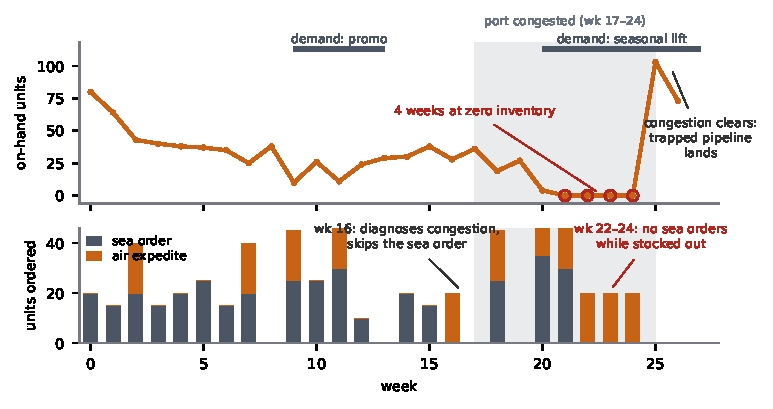
\includegraphics[width=\textwidth]{figures/fig3.pdf}
  \caption{\textbf{The freeze, week by week (Claude Sonnet 5, seed 1).}
  Top: on-hand inventory; the shaded band is the true port-congestion window
  (weeks 17--24) and the rugs above mark the true demand windows, none of
  which the agent observes directly. Bottom: units ordered by sea and by
  air each week. The agent diagnoses the congestion in week 16, its sea
  orders pile up behind the blocked port, and in weeks 22--24 it stops
  ordering by sea while holding zero inventory --- reasoning that the
  trapped pipeline is ample cover. When the congestion clears in week 25,
  the trapped orders land at once. Every series is parsed from the raw
  episode trace.}
  \label{fig:seed1}
\end{figure}

\paragraph{Exhibit A: freezing (Claude Sonnet 5, seed 1).} Week 16, on
diagnosing the congestion: ``Port congestion has spiked severely
(berth\_wait 10 days\ldots) \ldots\ I'll skip placing a new sea order this
week \ldots\ and reassess next week once conditions hopefully ease.''
Week 22, with zero on-hand inventory and a stockout in progress: ``Despite
the current 0 on-hand inventory, I already have a very large pipeline: 104
units in transit (arriving weeks 23--25) \ldots\ roughly 4--5 weeks of cover
\ldots\ ordering more now would only add to an already oversized pipeline,
incurring extra holding/in-transit costs and demurrage risk given
berth\_wait is still elevated (15 days).'' Weeks 21--24 all close at zero
inventory (\$660--\$823 per week).

\paragraph{Exhibit B: flailing (DeepSeek-V4-Pro, seed 25).} Week 4:
``Week 4: Disruption confirmed --- Suez counts crashed to 28/25 \ldots\ Cape
is now the only safe route. Locked freight at 1.02x for 4 weeks. Ordering 40
via Cape/spot \ldots'' Week 6, correctly closing the diagnosis: ``Week 6: Suez
reopening --- counts back to 56/56 \ldots'' By then the freight lock, air
expedite, and stacked orders are sunk; weekly costs run \$610--\$814 through
week 8, and the episode ends at \$7{,}950 total cost, skill $-1.45$.

\section{Agent Interface: Prompt and Observation Format}
\label{app:prompt}

\paragraph{Weekly observation.} The observation dictionary below is
serialized into the agent's context each week, exactly as produced by the
environment (a presentation-manifest key used only by the web frontend is
omitted). This example is week 10 of seed 1 under the base-stock policy:
the demand promo is active (point-of-sale 29 against a baseline of 20), the
lane is calm, and the symptom-blind policy has just taken a small stockout.

{\footnotesize\verbatiminput{appendix/obs_week10.json}}

\paragraph{System prompt (FAITHFUL arm).} The complete system prompt used
for all 200 runs is reproduced verbatim below. It specifies mechanics,
costs, tool semantics, and the latent structure of each factor, and
contains no strategy advice; its inclusion substantiates the rules-only
claim of Section~3.

{\footnotesize\verbatiminput{appendix/faithful_prompt.txt}}

% \bibliographystyle{plainnat}
% \bibliography{references}

\end{document}
